\section{Blockschema}
\tikzstyle{int}=[draw, fill=blue!20, minimum size=2em]
\tikzstyle{init} = [pin edge={to-,thin,black}]
\usetikzlibrary{positioning}
\begin{figure}[!h]
\centering
\begin{tikzpicture}[node distance=2.5cm,auto,>=latex']
    \node [draw, fill=blue!20, minimum size=10em] (a) {NEXUS 3};
    \node [draw, fill=blue!20, minimum size=10em,align=center] (b)[right of=a,node distance=15em] {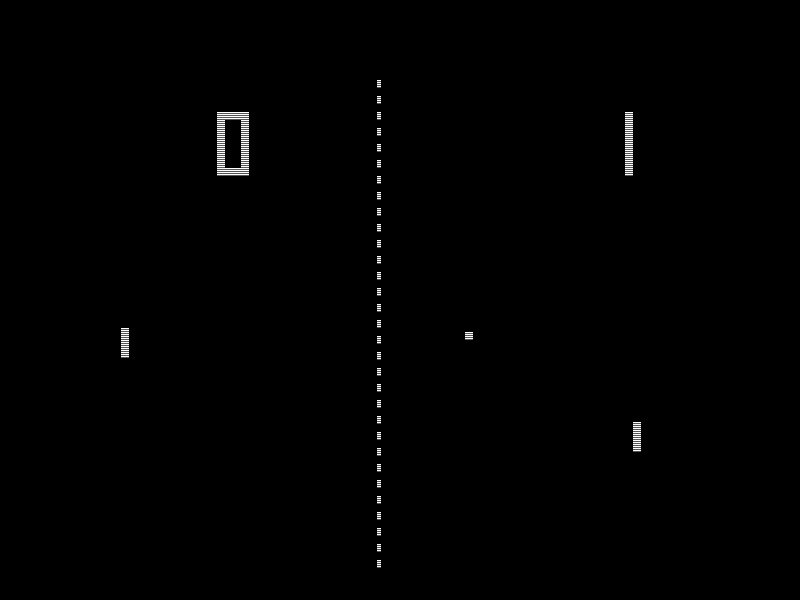
\includegraphics[scale=0.2]{../grafik/Pong.png} \\ VGA screen};
    \node [draw, fill=blue!20, minimum size=4em] (c) [left of=a,node distance=10em,anchor=north]{Joystick 1};
    \node [draw, fill=blue!20, minimum size=4em] (d) [above of=c,node distance=4.2em]{Joystick 2};
    \path[->] (a) edge node {VGA} (b);
    \path[->] (c) edge node {SPI} (c-|a.west);
    \path[->] (d) edge node {SPI} (d-|a.west);
\end{tikzpicture}
\end{figure}

